\chapter{Introduction and Background}
\label{chap:intro}

The First Nations people of Australia have lived here for over 65\,000 years and have oral traditions that highlight their understanding of variations in the brightness of stars. In particular, this knowledge encompasses the naked eye observations of the decades-long variability of three of the brightest equatorial stars, known in Western astronomy as Aldebaran, Betelgeuse and Antares \citep{hamacher_observations_2018}. In contrast to this, Western astronomy accepted the conclusions of Aristotle (350 BCE) for almost two thousand years that stars are static, with the exception of observations of supernovae. 

David Fabricius observed changes in the brightness of Mira in 1596 and confirmed stars were not static but could indeed be variable \citep{hoffleit_history_1997}. Our understanding of stellar variability has progressed significantly in the last century, both in terms of the variety of stars where we observe variability and the explanation for its existence. Henry Russell's 1918 address on variable stars stated `almost all variable stars are... giants...' with variability being a characteristic of the early life of a star \citep{payne-gaposchkin_development_1978}. These variable stars were limited to approximately 1\,700 examples divided into five classifications: novae, long-period variables (like Mira), irregular variables, Cepheids, and eclipsing stars. 

Today, the General Catalog of Variable Stars \citep{samus_general_2017} contains 117 distinct classes of variable objects, almost all belonging to the subset of variable stars and including stars of all evolutionary stages. This progress is the result of technological advances, from observations by eye through the adoption of photographic plates and finally to modern Charge-Coupled Devices (CCDs), providing increased precision in photometric measurements. Advances in the theoretical framework for stellar interiors, processes and evolution have also helped expand our knowledge of these variable classifications. The \Kepler{} space telescope provided photometry of micro-magnitude precision that helped revolutionize the study of stellar variability and drive advances in both observational and theoretical stellar physics.

This thesis presents a broad analysis of the open cluster members and the surrounding field stars within the nominal \Kepler{} field of view, focusing on the photometric variable stars. We begin with an introduction to key concepts for the work that follows: a brief summary of variable stars and their importance, the use of asteroseismology in understanding these stars, basic properties of the open clusters this thesis investigates, and the \Kepler~space telescope. Each chapter hereafter also contains a smaller, targeted literature review specific to the investigation contained within. Chapter 2 presents \Gaia~astrometric membership determinations for all stars within the fields of view of the nominal \Kepler~mission open clusters. We investigate the Red Giant solar-like oscillators in NGC\,6791 and NGC\,6819 as an ensemble based on this membership in Chapter 3; global asteroseismic properties of all cluster red giants that have measurable oscillations are presented, including new red giants and those with additional data. We also include variability classifications for stars we have re-classified as non-members in the red giant branch regions of the CMDs for these clusters. In Chapter 4 we present an in-depth study of a previously unknown variable we discovered within the NGC\,6791 superstamp image, classifying its variability type and presenting its suitability for future investigations of Ap magnetic fields. We conclude with a summary of the results of these investigations and provide avenues for future work in Chapter 6.

%Chapter 2 describes new stellar photometry we have extracted from the \Kepler~superstamp images of the open clusters NGC\,6791 and NGC\,6819, as well as basic properties of these variable stars. In Chapter 3 we study one of these previously unknown variables in greater depth, classifying its variability type and presenting its suitability for future investigations of Ap magnetic fields. Chapter 4 presents \Gaia~astrometric membership determinations for all stars within the fields of view of the nominal \Kepler~mission open clusters. We investigate the Red Giant solar-like oscillators as an ensemble based on this membership in Chapter 5; global asteroseismic properties of all cluster red giants that have measurable oscillations are presented, including new red giants and those with additional data. We conclude with a summary of the results of these investigations and provide avenues for future work in Chapter 6.

\section{Introduction to Variable Stars}

The physical phenomenon producing variations in the photometric brightness of an object can be used to create a classification scheme for variables. \citet{eyer_variable_2008} have produced a classification tree (reproduced here as Figure \ref{fig:variability_tree}) based on four levels of differentiation: (1) intrinsic vs extrinsic variability, (2) the type of object that is variable, (3) the physical phenomenon causing the variability, and (4) the grouping of similar variable objects.

\begin{figure}[htbp]
    \centering
    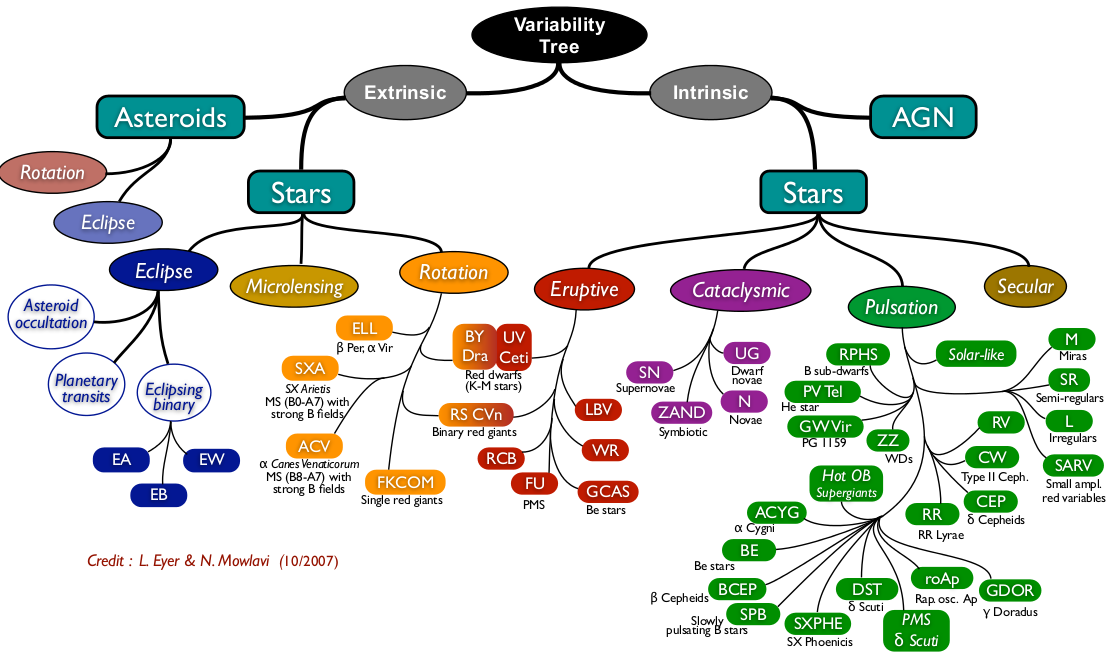
\includegraphics[height=0.78\linewidth,angle=-90]{Chapter1/variable_EyerMowlavi08.png}
    \caption[Variability classification tree]{Reproduction of \citet{eyer_variable_2008} classification tree of different variability types. Variable stars are the focus of this thesis so other variable objects at the second division level will not be discussed.}
    \label{fig:variability_tree}
\end{figure}

At the first division, intrinsic variables refer to stars where the variability is due to a physical process occurring withing the star itself. Extrinsic variability refers to cases where the geometry of the observer relative to the system leads to variability in its brightness. This thesis is only concerned with variable stars, so active galactic nuclei (AGN) and asteroids will not be discussed. 

The third differentiation is based on the specific physical phenomenon at the object that causes the variability. The largest intrinsic category is stellar pulsations, with almost all stars now known to exhibit this form of variability. Stellar rotation, showing different regions of the surface, and eclipsing stars make up the most common examples of extrinsic variability. At the lowest level, the different variable classifications are clustered together based on similar variability characteristics.

The classes are not all distinct at the lowest level, with some continuous transitions as the star passes from one evolutionary stage to another. To further complicate this classification process, variable stars may show signatures of more than one of these sources. (e.g. An eclipsing binary with a rotating and pulsating red giant component and a transiting exoplanet could show signatures belonging to four of these categories.) 

Detecting stellar variability at the lowest amplitudes relies on precise photometric measurements, preferably with continuous observations over long time periods.
There have been many missions and surveys over the past two decades dedicated to obtaining multi-epoch photometry, including both ground-based projects (e.g. \textsc{Macho}, \textsc{Ogle} (I, II, and III), PanSTARRS, ASAS, and HAT) and space-based telescopes (e.g. \Kepler, \Gaia, MOST, \textsc{CoRoT}, and \textsc{Tess}).

Figure \ref{fig:variability_tree} was produced primarily for the classification of variables found in the \Gaia~mission and so is biased towards the broader classification of variable objects. Solar-like oscillators are combined into a single object classification in this schema, yet they account for a large proportion of the pulsating stellar variable population and include main-sequence stars, sub-giants, and red giants. This classification further separates stellar objects at different evolutionary stages into completely separate classifications. For example, evolved red giant stars showing Mira-like pulsations show no common branches in the diagram with the solar-like oscillators they evolved from.

The introduction of photometric space-based telescopes to study solar-like stars (e.g MOST) and to search for exoplanets around them (e.g \Kepler, \textsc{CoRoT}, and TESS) have provided high-precision photometry with the quality and quantity necessary to detect these oscillations unambiguously \cite[][and references therein]{chaplin_asteroseismology_2013}. This data has revolutionised the study of stellar variability \cite[e.g.][]{aerts_asteroseismology_2010, di_mauro_review_2017, garcia_asteroseismology_2019}. 
% \todo{CHECK THESE REFERENCES!!}

\subsection{The importance of variable stars}

Variable stars are key to understanding stellar conditions beyond our Sun. Characterising eclipsing binaries, for example, provides: stellar masses of unrivalled precision \citep{torres_accurate_2010,rebassa-mansergas_accurate_2019}; orbital periods; eccentricities, and thus separations that can help constrain explanations of stellar phenomena (e.g. mass loss to a stellar companion vs mass loss from stellar winds). In large sample sizes they can also be used to constrain the proportion of stars in stellar systems, and have shown that more than 50\% of stars occur in binary systems \citep{raghavan_survey_2010, duchene_stellar_2013, moe_mind_2016, guszejnov_protostellar_2017}. These multiplicity rates have significant implications for stellar and planet formation models that are primarily based on the assumption of a solar system analogue.

Transiting exoplanets have become an active area of research over the past decade with the launch of high-precision photometric space-based missions revealing transit detections for a large number of stars \cite[eg.][and references therein]{zhu_about_2018,perryman_exoplanet_2018}. These detections enable studies of exoplanet occurrence rates \cite[eg.][]{narang_properties_2018}, characterisation in terms of relative planet size and density \citep{batalha_exploring_2014}, habitability zone rates \citep{gaidos_candidate_2013}, and population studies of potential Earth-like exoplanet candidates \citep{petigura_prevalence_2013, zhu_about_2018}.

Rotating variables refer to the subset of stars where rotation reveals the non-uniformity of their surfaces. The brightness variations arise because the rotation of the star changes the surface visible to the observer. In some rotating variables, star spots are the cause of this non-uniform surface brightness as they appear or disappear from the observer’s view. Stellar processes can cause star spots to change in size and temperature, producing secular changes that further complicate the analysis of these stars. Rotational variables are predominantly split into: $\alpha^2$ Canum Venaticorum ($\alpha^2$CVn) stars, where strong magnetic fields produce star spots; BY Draconis or UV Ceti stars that exhibit star spots and other chromospheric activity; and rotating ellipsoidal binary (ELL) stars, where orbital motions are responsible for changing the ellipsoidal stellar surface that is viewed. With the exception of ellipsoidal binaries, these stars provide insight into the strength and evolution of stellar magnetic fields \citep{berdyugina_starspots_2005}, and the impact of magnetic fields on stellar structure, behaviour, and evolution \citep{moss_dynamo_2004}. We discuss the newly-identified $\alpha^2$CVn star, KIC\,2569073, in \cref{chap:fluffy}.%We present new light curves and basic properties for some ellipsoidal binaries extracted from the \Kepler superstamps in \cref{chap:field} and discuss the investigation of the newly-identified $\alpha2$CVn star, KIC\,2569073, in \cref{chap:fluffy}.

Pulsating stars comprise a large fraction of intrinsic variable stars. These stars provide insight into the nature of stellar interiors, allowing us to determine fundamental stellar properties including density, radius, and mass \citep{chaplin_asteroseismic_2013, aerts_asteroseismology_2010, basu_asteroseismic_2017}. Changes in the brightness of stars caused by pulsations reveal internal stellar processes, including the specific driving mechanisms for different stellar types \cite[eg.][and references therein]{lenain_epsilon-mechanism_2006, welsh_koi-54_2011, aerts_asteroseismology_2010}, that in turn informs stellar evolutionary models \cite[eg.][]{garcia_observational_2015, houdek_surface_2017}. The next section discusses variable stars in more detail.

\section{Pulsating stars}

\cite{Eddington_internal_1926} asked ``What appliance can pierce through the outer layers of a star and test the conditions within?''. He believed that theory provided the best avenue for these investigations, although he cautioned against blind belief in these results without observational evidence. Today we know that asteroseismology of pulsating stars can provide that evidence. Pulsating variable stars are intrinsic variables where internal physical changes are responsible for the variations in their brightness. There are four main pulsation mechanisms that drive these intrinsic variations: the $\kappa$-mechanism \citep{eddington_cause_1941}, stochastic oscillations \citep{unno_stellar_1967}, convective blocking \citep{pesnell_new_1987}, and tidal excitation \citep{kumar_tidal_1995}.

\subsubsection{Excitation Mechanisms}

\cite{eddington_pulsation_1917} proposed treating stars as thermodynamic heat engines, where sound waves resonating through the stellar interior produce oscillations. Classical pulsators, such as Cepheids, RR Lyraes, rapidly oscillating Ap (roAp) stars, and $\delta$ Scuti stars, exhibit oscillations due to the $\kappa$-mechanism, a heat-engine mechanism based on opacity changes within the stellar envelope. When a shell of stellar material loses radiative pressure support, it collapses towards the star's centre, becoming compressed. These compressed regions restrict radiative transfer from the stellar core, storing additional flux \citep{zhevakin_physical_1963} that in turn ionizes regions of hydrogen or helium, increasing their opacity. This opacity increase drives the shell's expansion, which in turn causes cooling and decreases the opacity of the regions as they expand beyond the equilibrium point. The resulting oscillation around this equilibrium results in the observed pulsation variations \citep{king_pulsating_1968}.

Stochastic oscillations result from convective turbulence in the outer stellar envelope. These are randomly excited oscillations driven by turbulence in thick convective regions, where convective and pulsation timescales are closely correlated \citep{handler_asteroseismology_2013}. The stochastic perturbations result in global oscillations, or normal modes, at frequencies that correspond to standing waves. These modes have finite lifetimes due to damping and should only be excited in stars with lower effective temperatures than the cool edge of the classical instability strip. This boundary marks where convective envelopes are present. These stars are referred to as solar-like oscillators because the pulsation driving mechanism is the same in these stars as the mechanism in the Sun.

Convective blocking occurs in stars where the base of the convective zone is sharp and convective timescales are much longer than pulsation timescales. The transition from the radiative inner layer to the base of the convective envelope results in an increased opacity that drives pulsations. \cite{guzik_driving_2000} predicted that convection at the base of the envelope convective zone could not adapt to the more rapid pulsation changes, periodically blocking the radiative flux from the stellar interior, and resulting in g-mode oscillations. This mechanism dominates pulsations in late A and early F main sequence stars, called $\gamma$ Doradus pulsators.

Finally, binary stars in highly eccentric orbits experience large gravitational tidal forces during closest approach (periastron). These tidal forces can excite oscillations within the stellar interior, resulting in `heartbeat' stars \citep{thompson_class_2012}.

Pulsating variable stars are classified based on how the different pulsation driving mechanisms affect the photometry, and the frequencies of the oscillations these mechanisms produce. In more fundamental terms these classifications are based on the evolutionary state of the stars and their masses, which in turn determine the driving mechanisms. In some stars, known as hybrid oscillators, these fundamental properties result in multiple mechanisms simultaneously driving pulsations \cite[e.g.][]{antoci_excitation_2011}. 

\subsection{The HR Diagram and pulsating stars}

The Hertzsprung-Russell (HR) diagram depicts stellar populations based on their effective temperatures and luminosities, and provides a useful method for separating these pulsational variables based on their mass and evolutionary state. Figure \ref{fig:HRdiag} shows a typical HR diagram annotated with the most common pulsating variable classifications. Evolutionary tracks (solid lines) for 1\Msol \textendash{} 20\Msol stars are shown, with the 1\Msol track extended (dashed line) to the white dwarf evolutionary state. The classical instability strip (dotted lines) is also marked from the zero age Main Sequence (ZAMS) where the evolutionary tracks begin. The dominant observed pulsation modes (see Section \ref{chap:intro:astero}) in each variable class are shown, with p-modes (\textbackslash\textbackslash) and g-modes (//) marked by hashed lines, and solar-like oscillators (\textbackslash\textbackslash) classified separately. %????The dominant restoring forces for the observed pulsation modes at different evolutionary states are depicted as follows: opacity mechanisms driven within the second helium ionization zone are presented as diagonal hashes from top left to bottom right, stochastic oscillations are presented as horizontal hashes, convective blocking as diagonal hashes from top right to bottom left, 
%Luminosity can be difficult to calculate, particularly for the most distant stars, as it relies on precise distance determinations. The observational equivalent of this diagram is the colour-magnitude diagram (CMD) where colour replaces effective temperature and apparent magnitude replaces luminosity.

\begin{figure}[htbp]
    \centering
    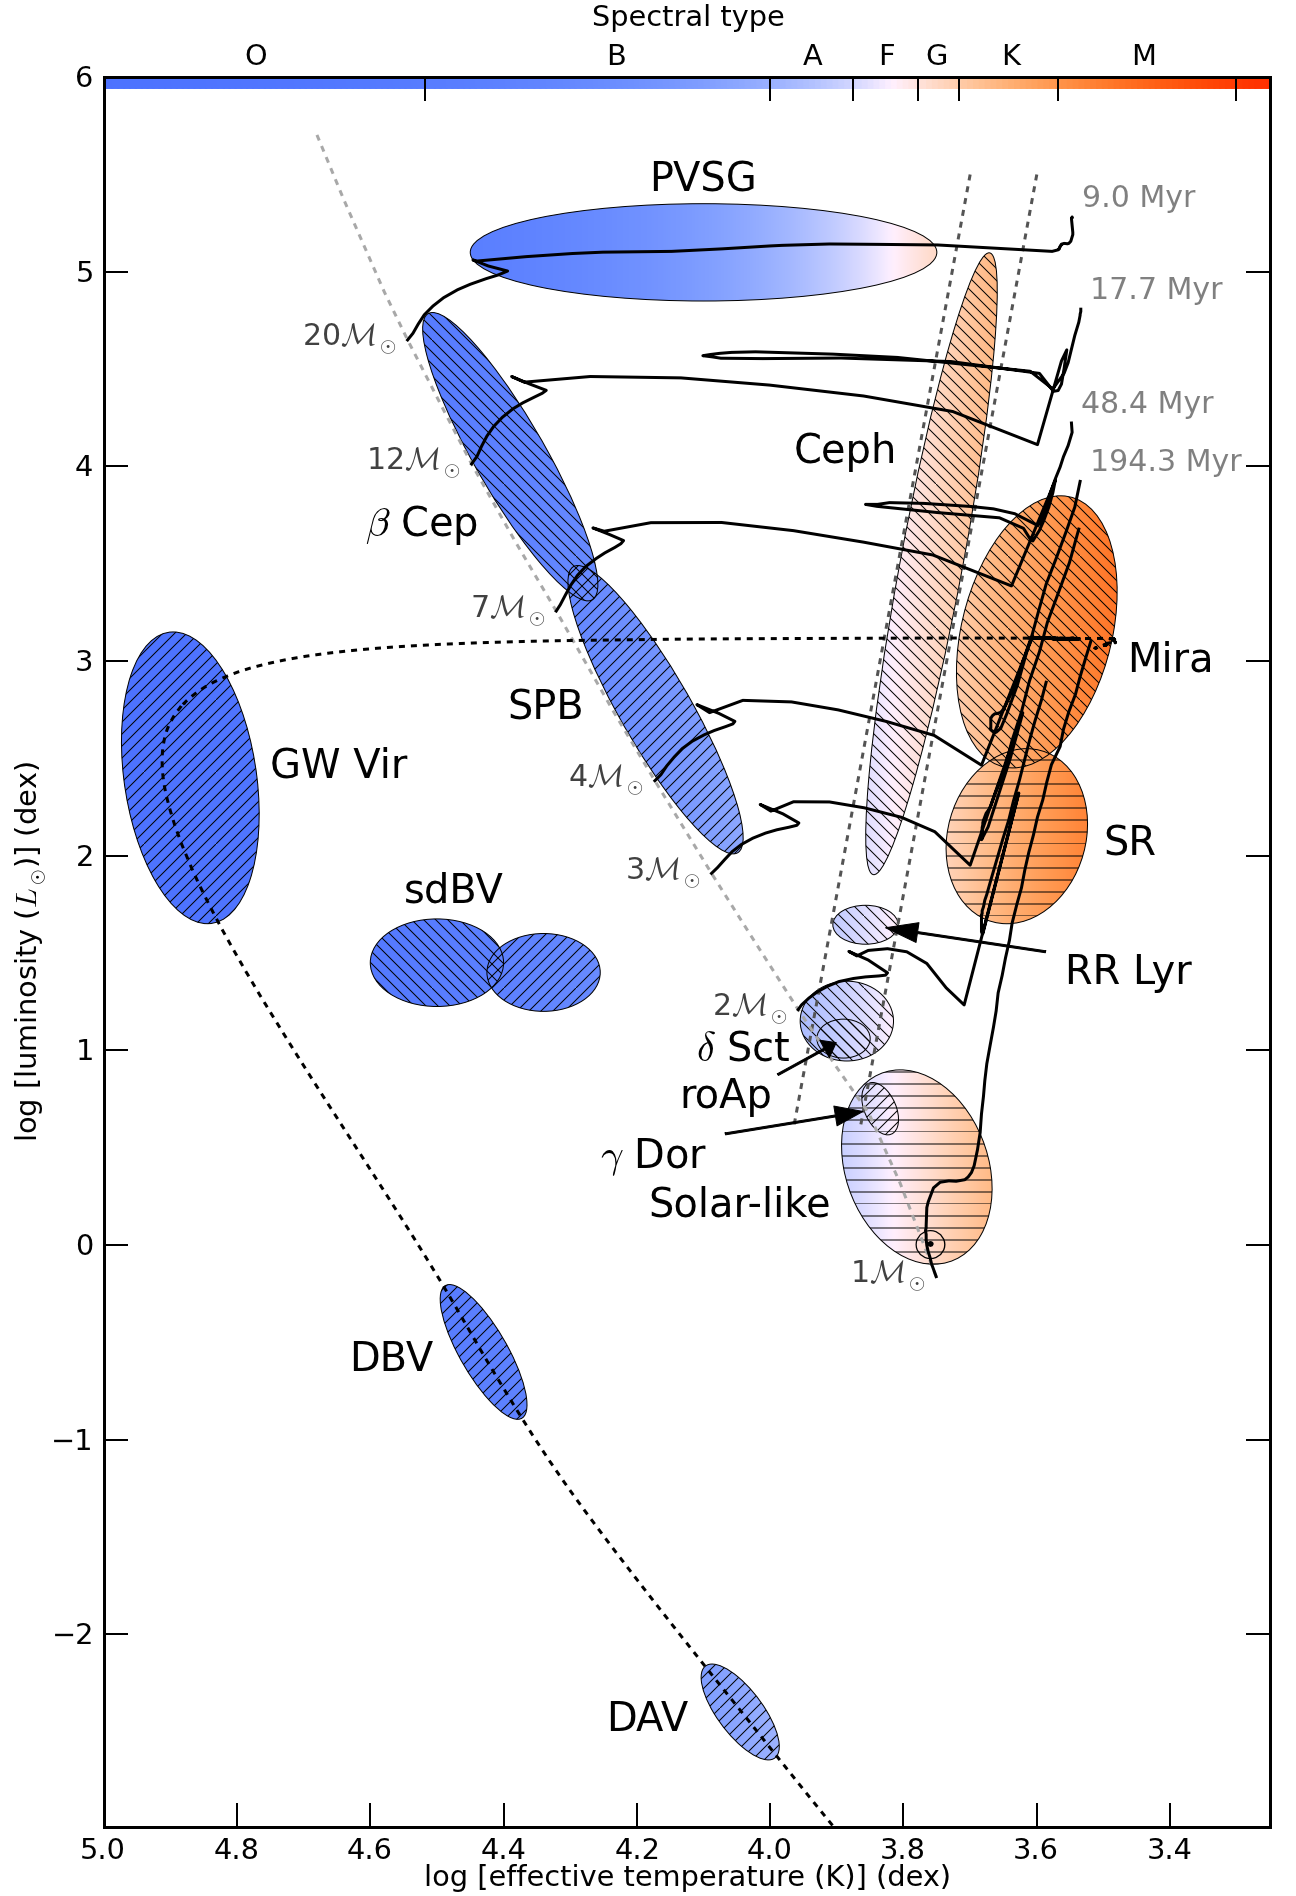
\includegraphics[width=0.88\linewidth]{Chapter1/HR_pulsational.png}
    \caption[Pulsational Hertzsprung-Russell Diagram]{Hertzsprung-Russell Diagram showing the most common categories of pulsational variables. Evolutionary tracks (solid lines) for a range of stellar masses are depicted, starting from the zero age main sequences (ZAMS). The classification category for the dominant pulsation modes (g-modes - // and p-modes - \textbackslash\textbackslash) at different evolutionary stages is also shown, with solar-like oscillators (\textbackslash\textbackslash) classified separately. Image Credit: P. Begroote, P. Papics}
    \label{fig:HRdiag}
\end{figure}

Almost all stellar evolutionary states, and thus almost all stars, exhibit oscillations. Stellar evolution results in stars crossing the HR diagram and passing between different instability regions where these pulsations are driven. The paths these stars follow are primarily determined by their initial mass and chemical composition, although internal mixing processes, magnetic fields, and mass transfer from binary interactions also have an affect. 

A large number of pulsational variables, including $\delta$ Scuti, roAp, RR Lyrae, and Cepheids, fall within the classical instability strip. This strip describes a region of the HR diagram through which some stars pass during their evolution. The $\kappa$-mechanism, acting within the helium partial ionisation zone, is predominantly responsible for stellar oscillations in this region \citep{king_pulsating_1968}. The boundaries are marked by the hot edge, where the helium partial ionization zones are located too close to the stellar surface for oscillations to be driven, and the cool edge, where outer convective layers damp pulsations from these zones too efficiently.

Beyond the cool edge of the instability strip lie the solar-like oscillators. The oscillations in solar-like stars are driven primarily by stochastic turbulence in the outer stellar envelopes. Solar-like oscillators include red giants, which are the most common variable star type within the old open clusters discussed in Chapter \ref{chap:red_giants}.

\subsection{Stellar Evolution}

As evolutionary stage plays such a significant role in the type of stellar oscillations observed, we provide a brief overview of stellar evolution and direct the interested reader to \cite{kippenhahn_stellar_2012} and \cite{christensen-dalsgaard_stellar_2002} for more in-depth explanations. We limit this overview to stars with $M \leq 9$\,\Msol.

\subsubsection{Star Formation}

Star formation occurs within dense molecular clouds of the interstellar medium (ISM). A cloud will collapse if the total mass is greater than the Jeans Mass, $M > M_J \propto T^{3/2} \rho^{-1/2} \mu^{-3/2}$, where $T$ is the temperature, $\rho$ is the mean density of the cloud, and $\mu$ is the mean molecular weight. The cloud undergoes isothermal collapse, fragmenting into clusters of protostars, with the converted gravitational energy being mostly radiated away. This contraction becomes adiabatic as the mean density of the cloud increases and it becomes more opaque and the temperature rapidly increases. When the protostar reaches hydrostatic equilibrium it enters the pre-main sequence and is located on the {\em Hayashi} track \citep{hayashi_stellar_1961}.

\subsubsection{Pre-Main Sequence}

At this point the pre-main sequence (pre-MS) star is fully convective and continues gravitational contraction, moving almost vertically down the HR diagram and decreasing in luminosity with an almost constant effective temperature. The more massive the protostar, the less time the star spends on the {\em Hayashi} track. The denser, more optically thick gas traps the radiation, and the internal temperature of the star begins to increase, becoming more transparent and thus enabling radiative transfer to dominate in the stellar core. As the radiative core grows, the luminosity becomes almost constant and the effective temperature begins to increase. The star is now moving horizontally to the left in the HR diagram, along the {\em Henyey} track.

Eventually the core temperature reaches $\sim10^6$\,K and the proton-proton (PP) chain reactions begin, with H fusing to form ${}^{2}$H, that in turn is converted to ${}^{3}$He. The high internal temperatures required for the onset of these reactions cause convective transfer to once again dominate in the core. For stars with masses less than $\sim1.1\,$\Msol{} the radiative core will return as soon as the PP chain reaction reaches equilibrium and the star reaches the zero age main sequence (ZAMS).

\subsubsection{Main Sequence}

The main sequence (MS) is defined by core hydrogen burning, with stars spending \texttildelow{}90\% of their lifetimes in this phase. Initial stellar mass is the defining factor for stellar lifetimes, although metallicity can also play a significant role. An initial stellar mass on the ZAMS, $M_{\mathrm{ZAMS}}$, of less than 0.08\,\Msol{} marks the low-mass boundary below which the PP chain will never reach H equilibrium, producing brown dwarfs. Stars with 0.08\,\Msol$ \leq M_{\mathrm{ZAMS}} \leq $ 0.35\,\Msol{} will remain fully convective for their lifetimes. Stars with 0.35\,\Msol{} $\leq M_{\mathrm{ZAMS}} \leq $0.5\,\Msol{} leave the MS as helium white dwarfs (WDs). Stars with an initial mass between 0.35\,\Msol{} and 1.1\,\Msol{} have cores dominated by radiative transfer, surrounded by a convective envelope.

If the stellar mass is higher than $1.1\,$\Msol, the core will remain convective for at least part of the MS phase because the CNO catalytic cycle, which is much more temperature sensitive than the PP chain, dominates the hydrogen fusion reactions. The convective cores in these stars mix hydrogen from the radiative shell into the core, helping to prolong their MS lifetimes. The radiative shell surrounding the convective core is further out for higher masses and the convective outer envelope disappears above 1.5\,\Msol{}. 
For these higher mass stars, internal mixing of the convective core helium content creates a sharp discontinuity in mean molecular mass, $\mu$, at the convective-radiative boundary, that in turn results in a lower mean density. These stars evolve to the right in the HR diagram, decreasing in effective temperature as the star expands with only a slight increase in luminosity. The star then rapidly contracts when the core hydrogen content is exhausted, creating the `hook'. In comparison, stars with a radiative core like the Sun have a continuous distribution in mean molecular mass, so show no hook feature. Stars reach the terminal age main sequence (TAMS) once their core hydrogen is exhausted, which for stars of mass between 0.5\textendash{}2.3\,\Msol{} is typically on the order of 1\textendash{}50\,Gyrs.

\subsubsection{Subgiants}

Once hydrogen is exhausted in the core, hydrogen burning occupies a shell moving radially outwards that surrounds a growing inert helium core. This is referred to as the subgiant branch, where stars spend \texttildelow{}5\% of their lifetimes. During this evolutionary stage the star evolves to the right in the HR diagram. The energy of fusion of the hydrogen shell layer is transferred almost entirely to the expansion of the envelope, resulting in a drop in the stellar effective temperature. Eventually lower mass stars ($0.5$\,\Msol{}$ \leq $ M $ \leq 2.3$\Msol{}) develop cores that are too massive to be supported and they become degenerate. At this point the rate of hydrogen fusion within the stellar envelope increases dramatically and the star moves to the Red Giant Branch (RGB). For more massive stars, $M \geq 2.2$\,\Msol{}, the core temperature is much higher so the mean stellar density is lower. These stars do not develop a degenerate helium core.

\subsubsection{Red Giants and later evolution}

The expanding hydrogen-burning shell deposits additional helium on the inert core, increasing its mass, which in turn causes the core to contract and heat up. This additional heat increases the shell temperature, compressing the hydrogen-burning shell and thus increasing the rate of energy production. The difference between the density of the inert helium core and the envelope increases until they become decoupled. At this point the stellar luminosity depends only on the helium core mass.

The convective envelope penetrates the stellar interior, where the chemical composition has been modified by the main sequence reactions. Convection dredges this material to the surface, leaving behind a region of discontinuous chemical composition. When the hydrogen burning shell reaches this region, the change in the mean molecular mass temporarily results in a decrease of the stellar luminosity, creating the RGB bump. This only occurs for stars of mass lower than 2.2\,\Msol{}, where the hydrogen shell reaches the dredge up zone prior to the helium core igniting.

The convective zone continues to deepen and the star follows the {\em Hayashi} track in reverse, increasing in luminosity. The stellar radius grows as the star climbs the red giant branch until the core temperature is high enough ($\sim10^8$\,K) for the onset of helium burning. At this point the star is at the tip of the RGB, with a radius approximately 200 times larger than its MS radius. Stars on the RGB have temperatures ranging from T$_\mathrm{eff}$ \texttildelow{}3500\,K \textendash{} 5000\,K.

Lower mass stars (0.5\,\Msol$ \leq M_{\mathrm{ZAMS}} \leq $ 2.2\,\Msol{}) have degenerate helium cores that continue growing through the RGB phase until a critical core mass is reached at \texttildelow{}0.45\,\Msol{}. At this point the helium ``flash'' occurs as a runaway thermal process. The pressure of the highly degenerate core is independent of the temperature and thus increasing temperature at this point does not trigger expansion and cooling. Instead, the enormous energy produced in this flash is absorbed by the layers surrounding the degenerate core. This flash and potentially further core sub-flashes lift the core degeneracy. As the convective core expands, the stellar envelope contracts and the luminosity decreases, with the star entering the horizontal branch (HB) or the red clump (RC), where core helium burning occurs. Stars with masses slightly higher than 2.2\,\Msol{} don't have a degenerate helium core, so undergo a more gradual helium ignition phase, forming the secondary red clump at lower luminosities.

Upon core helium exhaustion, the star begins ascending the asymptotic giant branch (AGB), closely following the RGB in the HR diagram. In this phase the star is undergoing shell hydrogen and helium burning and exhibits thermal `pulses' as corresponding shells ignite and are exhausted. Strong stellar winds and the corresponding substantial mass loss are a characteristic of these stars, ultimately resulting in the formation of a white dwarf for stars near solar mass surrounded by a short-lived planetary nebula.

\subsection{Asteroseismology}
\label{chap:intro:astero}
Asteroseismology is the study of stellar oscillations. It allows us to indirectly look below the photosphere and study the interiors of pulsating variable stars by making precise measurements of their surface brightness or radial velocity over long periods of time. This thesis is concerned with asteroseismology based solely on photometric measurements, so this shall form the focus of the following discussion. The surface brightness varies due to perturbations of the photosphere caused by standing waves, or pulsations, within the star. These standing waves are classified as either pressure modes (p-modes) or gravity modes (g-modes) based on their restoring forces. Pressure modes are acoustic waves where pressure acts as the restoring force, whilst g-modes are restored by buoyancy. 

These modes propagate through different regions of the stellar interior, penetrating to different depths depending on the stellar structure and density. Figure \ref{fig:modes} shows the propagation paths of p-modes (left) and g-modes (right) within a Sun-like star. Since different modes penetrate different stellar layers, the combined information allows us to study the star's internal structure.

Individual modes can be defined using three quantum numbers: the radial order, $n$, the angular degree, $l$, and the azimuthal order, $m$ where $-l \leq m \leq l$. These integers describe the number of radial nodes within the star ($n$), the number of surface nodes ($l$), and the number of surface nodes that correspond to lines of latitude ($m$). We can model these oscillation modes as combinations of spherical harmonics, described by Equation \ref{eqtn:spherical_harmonics}, where $N^m_l$ is the normalisation factor applied to the associated Legendre polynomials, $P^{|m|}_l$ \citep{handler_asteroseismology_2013}.

\begin{equation}
    Y^m_l (\theta,\phi) =N^m_lP^{|m|}_l\cos(\theta)e^{im\phi}
    \label{eqtn:spherical_harmonics}
\end{equation}

\begin{figure}
    \centering
    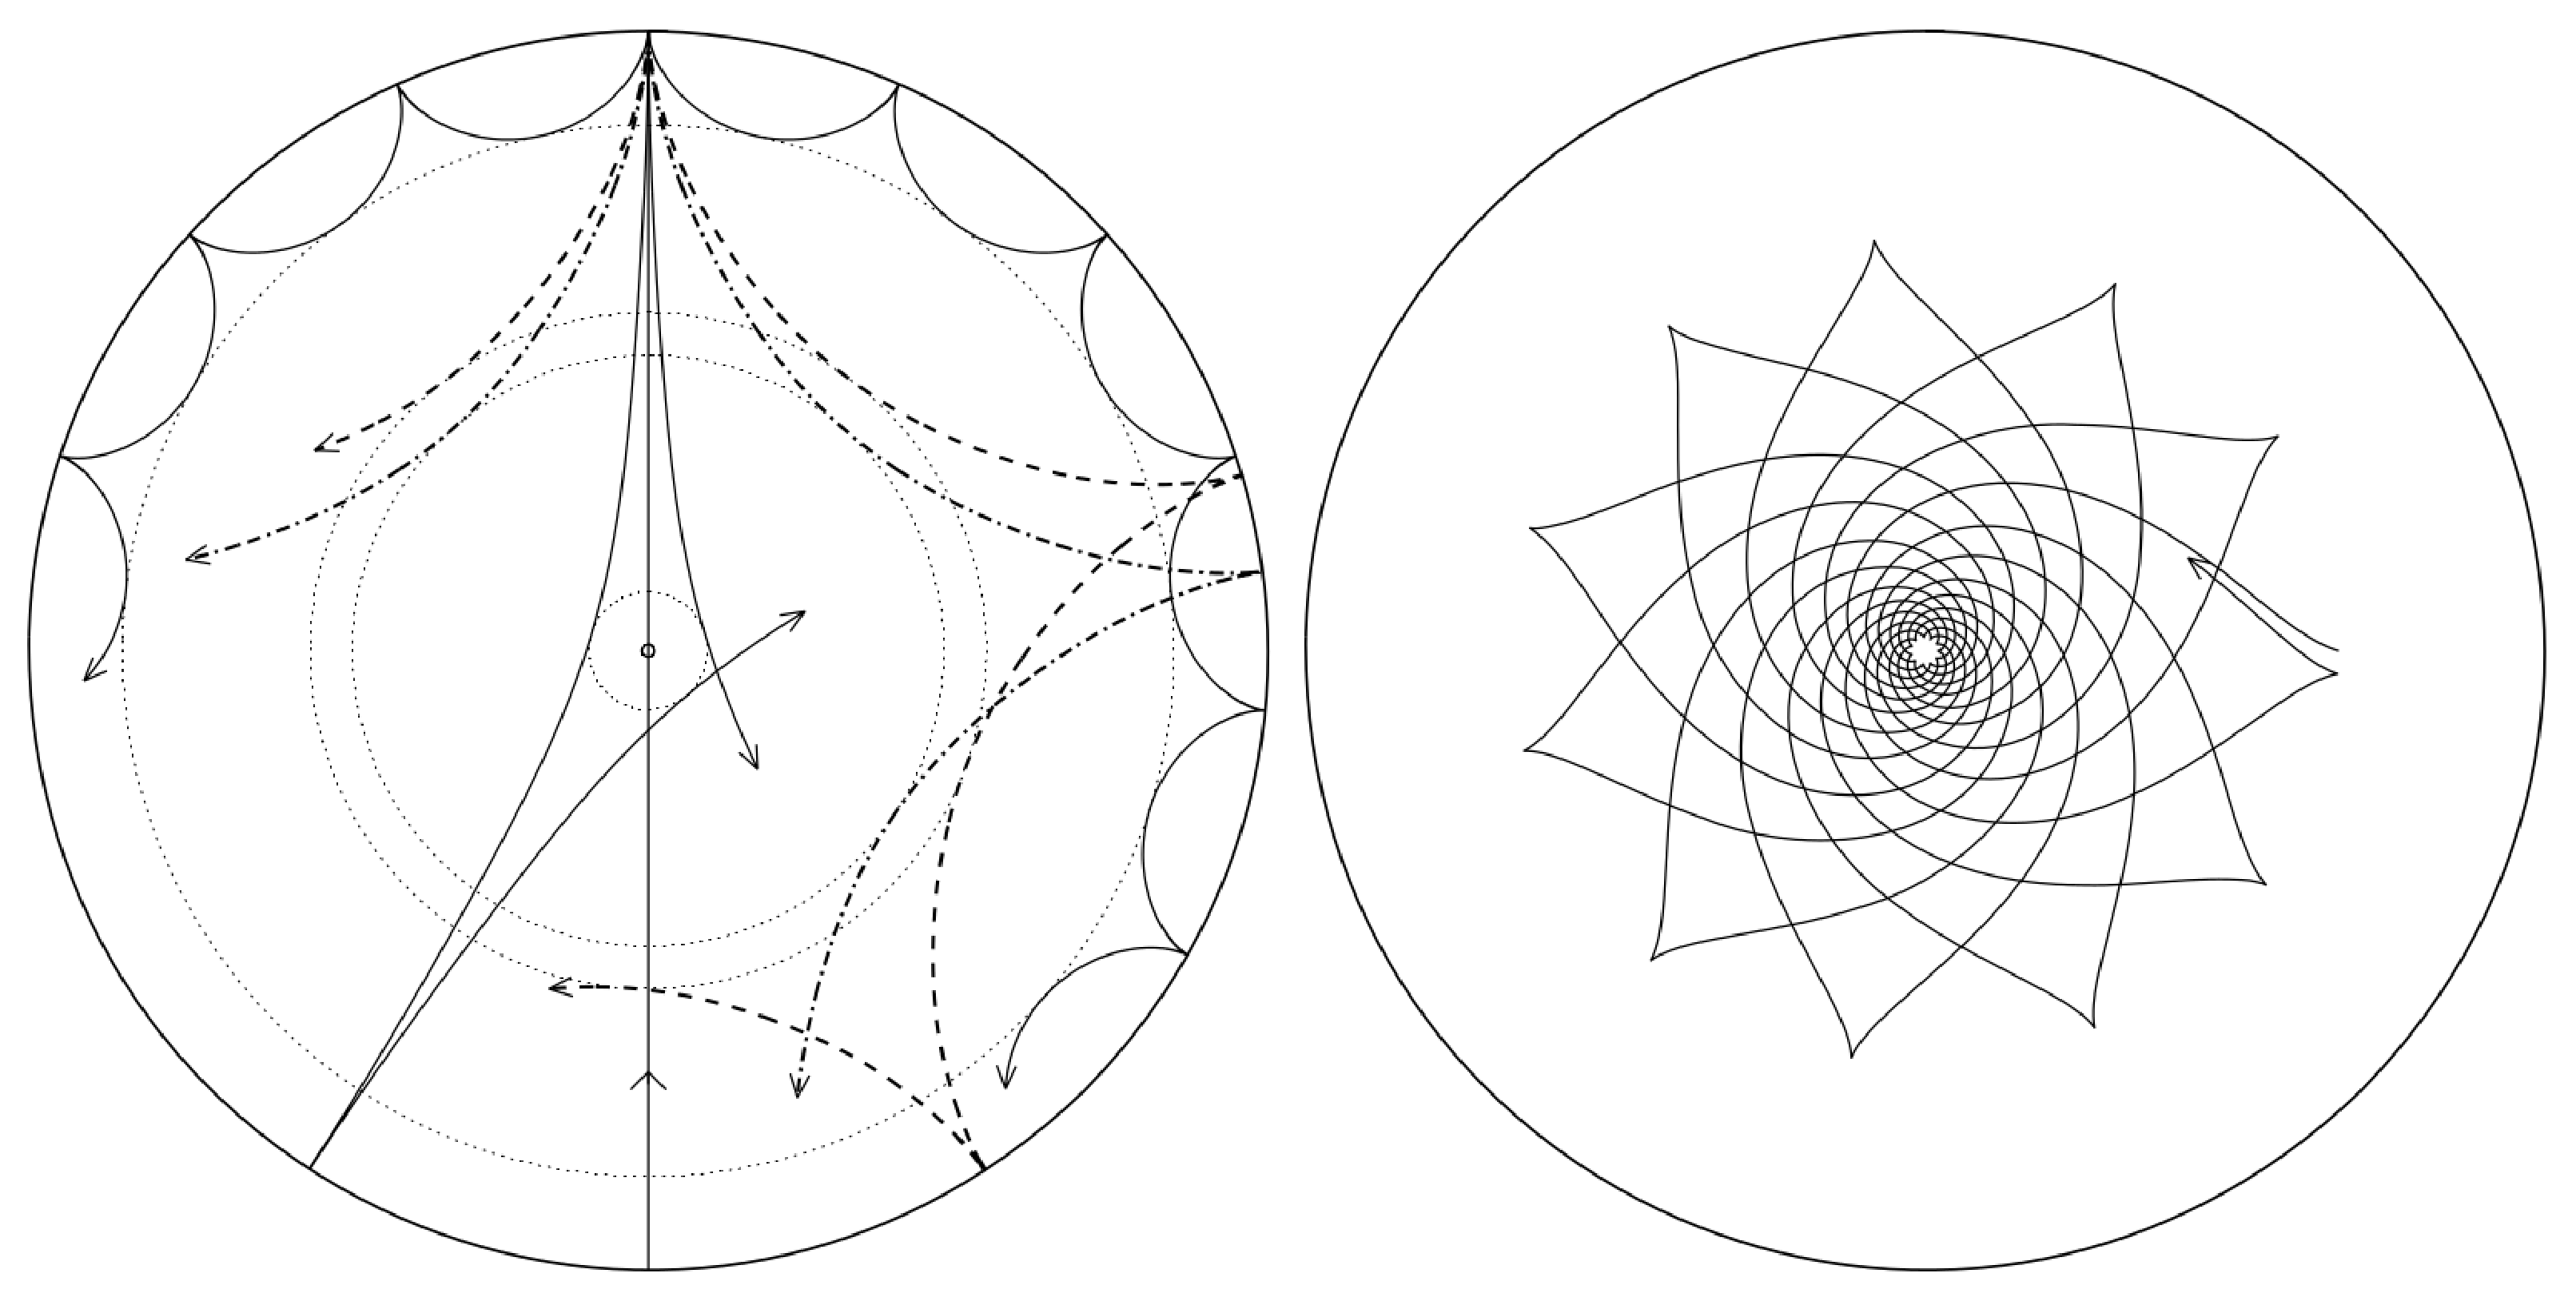
\includegraphics[width=\linewidth]{Chapter1/modes.eps}
    \caption[Propagation of p-modes and g-modes in a solar-like star]{Propogation of p-modes and g-modes in a Sun-like star, with p-modes (left) of lower angular degree penetrating deeping into the stellar interior and g-modes (right) trapped within the stellar core. Image Credit: \cite{aerts_asteroseismology_2010}}
    \label{fig:modes}
\end{figure}

For stars other than the Sun, the lack of spatial resolution of the stellar surface results in geometric cancellation effects, limiting the resolution of stellar modes to those of low angular degree \citep{aerts_asteroseismology_2010}. Typically this means only modes of $l \leq 2$ are visible, although for some stars $l = 3$ modes can also be observed. Figure \ref{fig:spherical_harmonics} shows the first ten spherical harmonics with angular degree $0 \leq l \leq 3$ and prograde modes of azimuthal order $0 \leq m \leq 3$. The retrograde modes have been omitted for conciseness as they only differ from the prograde modes by a phase change.

\begin{figure}
    \centering
    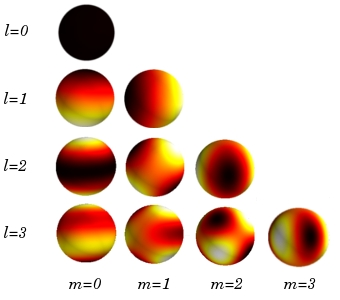
\includegraphics[width=0.45\linewidth]{Chapter1/spherical_harmonics.png}
    \caption[Spherical harmonics and prograde modes]{Spherical harmonics of angular degree $0 \leq l \leq 3$ and prograde modes of azimuthal order $0 \leq m \leq 3$. Retrograde modes have been omitted for conciseness. The colour scale shows the maxima (black) and minima (white) displacements of the stellar surface. The $l = 0$ mode corresponds to the radial contraction and expansion of the star. Figure from Honours thesis (Drury, 2013).}
    \label{fig:spherical_harmonics}
\end{figure}

%\cite{murphy_investigating_2014} define the azimuthal order, with positive $m$ values referring to prograde modes that have higher frequencies in the observer's reference frame than retrograde, or negative $m$ value, modes. 
In the spherically symmetric case, modes with a given radial order and angular degree have the same oscillation frequencies, with azimuthal order having no effect. If this symmetry is broken by strong magnetic fields or stellar rotation, however, we observe mode splitting that can allow measurements of properties that are otherwise difficult to obtain, such as stellar inclination angle \citep{corsaro_spin_2017}. % We will revisit this in Chapter \ref{chap:red_giants}.

\subsubsection{Observations}

The analysis of stellar oscillation modes requires precise photometric measurements over long periods of time. Figure \ref{fig:lightcurve_examples} presents light curves for a variety of different variable stars. Only the highest amplitude oscillations can be clearly observed in these light curves. Asteroseismic analyses are typically conducted in the frequency regime by taking Fourier transforms of the light curves. This is extremely useful for identifying and analysing the individual oscillation modes present. Figure \ref{fig:powerspec_examples} shows the power spectra corresponding to the light curves in Figure \ref{fig:lightcurve_examples}.

\begin{figure}[p]
    \centering
    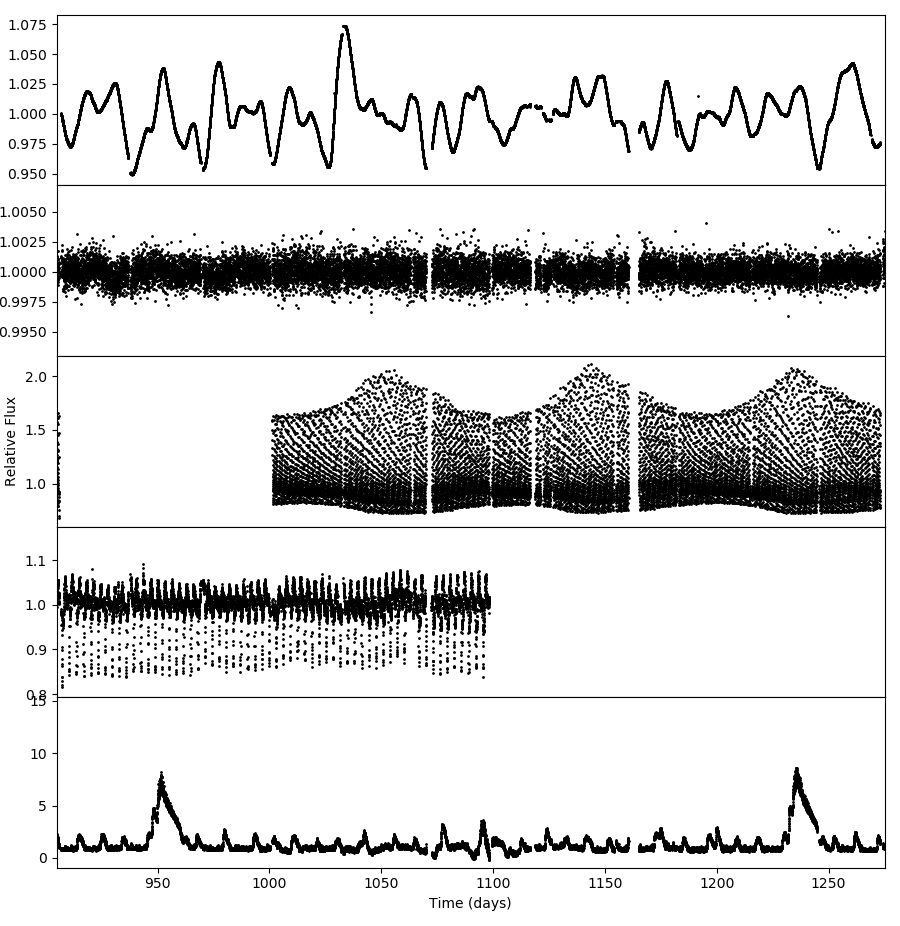
\includegraphics[width=\linewidth]{Chapter1/lightcurves.png}
    \caption[Light curves of variable stars]{Variable stars' light curves for: (a) highly evolved, high luminosity red giant, (b) low luminosity red giant, (c) RR Lyrae, (d) eclipsing binary, (e) ellipsoidal binary, and (f) nova variable star.}
    \label{fig:lightcurve_examples}
\end{figure}

\begin{figure}[p]
    \centering
    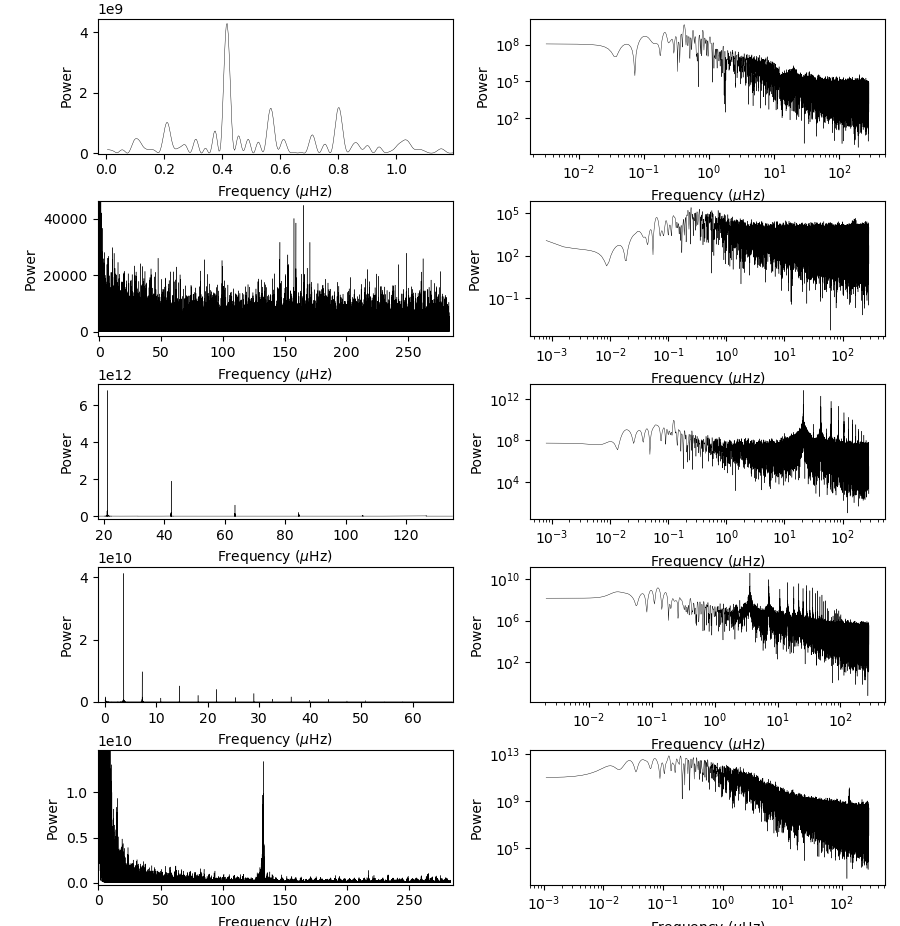
\includegraphics[width=\linewidth]{Chapter1/powerspectra.png}
    \caption[Power spectra for light curves of variable stars]{Power spectra for the light curves in Figure \ref{fig:lightcurve_examples} zoomed to the prominent features (left) and log-log scaled (right). It should be noted that nova variables are typically not investigated in the Fourier regime but this example is included here for comparison.}
    \label{fig:powerspec_examples}
\end{figure}

Photon noise is one of the dominant sources of error in photometry and is proportional to $\sqrt{\mathrm{N}}$, where N is the number of photons recorded. The longer the integration time of these observations the lower the photon noise and the easier it is to distinguish oscillation modes. Longer integration times however, must be balanced against the need for observations that are short enough for the variability to be resolved. 

When the individual modes in solar-like oscillators are resolved they can be well described by Lorentzian profiles

\begin{equation}
    L(\nu) = \cfrac{1}{\pi} \cfrac{\tfrac{1}{2} \Gamma}{(\nu-\nu_0)^2 + (\tfrac{1}{2} \Gamma)^2}
\end{equation}

\noindent where $\Gamma$ is the width of the profile. In resolved modes, the width is inversely proportional to the mode lifetime and the height is proportional to the amplitude of the mode, convolved with any geometric effects. If the mode's lifetime is similar to or greater than the observational timescale (ie. it is coherent) the mode will not be resolved. In this case the mode tends from a Lorentzian profile towards a $|$sinc$|$ profile.


\section{Open clusters}
\label{sect:litrev_ocs}
Open clusters are typically characterised as sparse, loosely gravitationally-bound stellar populations located primarily in the Galactic disk \citep{friel_old_1995, dias_proper_2002, kharchenko_global_2013, cantat-gaudin_clusters_2020}. Older open clusters tend to be more densely populated, with hundreds to thousands of members, compared to younger clusters that comprise a few tens to hundreds of members. These older open clusters also tend to be located at greater distances from the Galactic disk, where the probability of collisions with large molecular clouds, which disperse cluster members among the galactic field population, are lower \cite[][and references therein]{gieles_star_2006}. %\todo{Get reference from pad on bookshelf/in paper box?} 
Tidal disruption, disk and bulge shocking, and stripping from Galactic field interactions are also responsible for the dissolution of stellar cluster members into the field population \citep{marchi_search_2006}. All of these processes are stronger in the Galactic disk.%\todo{Check this statement}

It is usually assumed that stellar clusters form from a single nebula and consist of coeval, isometallic, cospatial and comoving members \citep{baade_resolution_1944}, with initial stellar mass being the primary parameter that differentiates members. \citet{mould_stellar_1982} showed that the metallicity and kinematics of cluster members are unchanged by stellar and galactic evolution, making cluster members ideal probes for a wide range of astrophysical investigations (e.g stellar interiors and atmospheres \citep{miglio_asteroseismology_2012, corsaro_asteroseismology_2012}, stellar evolution \citep{kalirai_star_2010, jilkova_origin_2012}, asteroseismic scaling relations \citep{stello_amplitudes_2011}, cosmology \citep{krumholz_star_2019}, Galactic evolution \citep{de_grijs_revolution_2010,boesgaard_old_2015}, and disk and planet formation \citep{bonnell_planetary_2001, meibom_same_2013}).

In terms of stellar evolutionary studies, having fewer free parameters for modelling cluster members allows the analysis to be conducted as a uniform ensemble, with a few exceptions resulting from rotation, magnetic field interactions and binarity \citep{carroll_introduction_2006}. Whilst globular clusters may experience multiple stellar formation epochs, this is not the case for open clusters \citep{li_stellar_2016}, which are instead well-described by a single isochrone (a composite of coeval theoretical evolutionary tracks for different initial mass values) transformed to an observational colour-magnitude diagram (CMD). Photometric observations of cluster members reveal outliers from these isochrones, with binarity being perhaps the most common cause \citep[e.g.][]{duquennoy_multiplicity_1991, murphy_finding_2018}, resulting in apparent magnitudes of up to 0.75\,mag brighter for unresolved binaries.

This thesis will focus on the four open clusters located in the nominal \Kepler field of view: NGC\,6791, NGC\,6819, NGC\,6811, and NGC\,6866. These clusters span a range of ages and metallicities. Table \ref{tab:cluster_properties} presents a summary of the global cluster properties.

\begin{table}[h]
    \setlength\tabcolsep{10pt}
    \centering
    \begin{tabular}{lcccc}
        \hline
                        & NGC 6791 & NGC 6819 & NGC 6811 & NGC 6866 \\
        \hline
        \hline
        RA                      & 19:20:53 & 19:41:18 & 19:37:17 & 20:03:55 \\
        Dec                     & +37:46:18 & +40:11:12 & +46:23:18 & +44:09:30 \\
        Distance (kpc)          & 4.1 & 2.3 & 1.2 & 1.45 \\
        Age (Gyr)              & 8.5 & 2.4 & 0.86 & 0.705 \\
        Metallicity [Fe/H]      & 0.34 & 0.09 & 0.04 & $-$0.1\\
        % Radius                  &  &  &  & \\
        %  - Core                 &  &  &  & \\
        %  - Tidal                &  &  &  & \\
        %  - Limiting             &  &  &  & \\
        %  Population             &  &  &  & \\
        \hline
        
    \end{tabular}
    \caption[A summary of the global properties of the four open clusters in the nominal \Kepler field of view]{A summary of the global properties of the four open clusters in the nominal \Kepler field of view; NGC\,6791, NGC\,6819, NGC\,6811, and NGC\,6866. Cluster positions and distances are sourced from WEBDA. Age and metallicity are sourced from the references included above. In the case of NGC\,6791, where little agreement exists between authors, values close to the median were selected for this table.}
    \label{tab:cluster_properties}
\end{table}

\subsection{NGC 6791}

NGC\,6791 is one of the oldest, most massive, and most metal-rich clusters in the Milky Way and has thus been extensively studied. Despite this, there is little agreement between authors concerning its basic parameters. Its metallicity has been reported as ranging from $[\mathrm{Fe/H}] = +0.29 \pm 0.03$ (random) $\pm 0.07$ (systematic) to $+0.45 \pm 0.04$\,dex, with the likely difference originating in the different reddening values used by the studies \cite[eg.][and references therein]{villanova_ngc_2018, cunha_sodium_2015}.

The age of the cluster is similarly difficult to obtain by the typical process of isochrone fitting due to differential reddening across the cluster \citep{brogaard_age_2012}. \cite{wu_asteroseismic_2014} has compiled a literature overview that lists 16 studies in the last two decades that have provided age determinations for NGC\,6791 ranging from 6.2 to 12\,Gyr, with an average age of \texttildelow{}8\,Gyr that agrees closely with the latest determination of $8.5 \pm 0.12$\,Gyr by \cite{hoyman_analysis_2019}. This overview provides the related distance moduli and reddening values for these studies with mean values of $(m-M)_V \sim 13.44$\,mag and $E(B-V) \sim 0.13$\,mag. 

\cite{king_color-magnitude_2005} and \cite{basu_sounding_2011} both calculated the heliocentric distance for NGC\,6791 to be \texttildelow{}4.1\,kpc, implying it is located \texttildelow{}1\,kpc above the Galactic plane \cite[see also ][]{cantat-gaudin_gaia_2018,grundahl_new_2008}. \cite{villanova_ngc_2018} concluded this cluster probably originated in the Galactic bulge, with its present location resulting from radial migration. 

In addition to these anomalous open cluster properties, NGC\,6791 is highly studied for its diverse stellar populations, including hot blue stars, white dwarfs spanning the length of the cooling sequence, highly variable stars including a cataclysmic variable, and multiple binary systems. These studies have led to changes in our understanding of stellar evolution. For example, \cite{bedin_reaching_2008} reported an age discrepancy of 2\,Gyr for the faint white dwarf population that was resolved by revisions to the theoretical white dwarf evolutionary path based on internal processes \citep{garcia-berro_white_2010}. The red giant branch population has also been extensively studied, particularly through the use of \Kepler{} data. \cite{basu_sounding_2011} determined the average RGB mass for NGC\,6791 to be $1.2 \pm 0.01$\,\Msol{} and \cite{brogaard_age_2012} found the less-evolved RGB stars to have masses of $1.15 \pm 0.02$\,\Msol{}. Further details on the RGB stars are contained in \cref{chap:red_giants}. These studies all rely on cluster membership determinations, which are discussed in more detail in \cref{chap:membership}.

\subsection{NGC 6819}

NGC\,6819 is much younger than NGC\,6791 and is considered a richly-populated, intermediate-age open cluster, with an age of $\sim$2.4\,Gyr \cite[eg.][and references therein]{handberg_ngc_2017, bedin_hubble_2015, basu_sounding_2011}. Unlike NGC\,6791, there is good agreement for the basic properties of NGC\,6819. \cite{bragaglia_metal_2001} determined the metallicity to be near-solar or slightly super-solar with $[\mathrm{Fe/H}] = +0.09 \pm 0.03$\,dex \cite[see also;][]{slumstrup_[y/mg]_2017}. \cite{ak_ccd_2016} presented a summary of published values for the distance and reddening of this cluster, along with their calculated values of $2.3$\,kpc and $E(B-V) = 0.130 \pm 0.035$\,mag. This value is in good agreement with the distance modulus of $(m-M)_0 = 11.83 \pm 0.14$\,mag calculated by \cite{wu_new_2014}.

These consistent values allow tight constraints to be placed on the cluster population. These tight constraints allow for stellar models to be computed on a smaller range of stellar parameter values, compared to those needed for modelling the stellar population of NGC\,6791, and thus allow for more precise investigations of stellar evolution. \cite{kalirai_initial-final_2008} used photometry and high-resolution spectroscopy to constrain the initial-final mass relation for cluster white dwarfs that, in turn, informs our understanding of how mass is lost in the 99\% of stars that end their evolution in this state. Studies of the radial velocities of cluster members have also shown no evidence of cluster rotation \citep{kamann_linking_2018}, despite conclusions to the contrary from the analysis of red giant oscillation mode splittings \citep{corsaro_spin_2017}.

\subsection{NGC 6811}

NGC\,6811 is a young sparse open cluster with an age of $\sim 0.86$\,Gyr \citep{janes_ngc_2013}. \cite{sandquist_age_2016-1} obtained a distance modulus of $(m-M)_V = 10.37 \pm 0.03$\,mag and a reddening of $E(B-V) = 0.07 \pm 0.02$ for NGC\,6811, corresponding to a heliocentric distance of $\sim 1.2$\,kpc. \cite{molenda-zakowicz_spectroscopic_2014} determined the metallicity of NGC\,6811 to be essentially solar, with $[\mathrm{Fe/H}] = +0.04 \pm 0.01$\,dex, and identified a number of cluster binaries and red giants.

Few studies of this cluster had been conducted prior to the \Kepler{} mission, with the exception of membership determinations (see \cref{chap:membership}) and searches for highly variable stars \citep{van_cauteren_search_2005, luo_variable_2009}. \cite{arentoft_convective-core_2017} used asteroseismic analyses of the 8 red giant cluster members to provide constraints on convective-core overshooting and oscillation mode suppression in stars of $2$\,\Msol{}. \cite{curtis_temporary_2019} have also provided evidence for low-mass stars in NGC\,6811 halting their evolutionary rotational spin-down, and providing a possible explanation for deviations in gyrochonology relations with respect to low-mass stars. The \Kepler{} space mission has also detected two sub-Neptune planets in NGC\,6811 \citep{meibom_same_2013}, taking the current total to four known exoplanets within clusters.

\subsection{NGC 6866}

NGC\,6866 is the youngest of the open clusters in the nominal \Kepler{} field of view, with an age between $479$\,Myrs and $705 \pm 170$\,Myrs \citep{janes_open_2014, gunes_astrophysical_2012}. \cite{bostanci_comprehensive_2015} determined the metallicity of this intermediate-age open cluster to be approximately solar, with $[\mathrm{Fe/H}] = -0.10 \pm 0.13$\,dex. The cluster has a calculated distance modulus of $(m-M)_0 = 10.98 \pm 0.24$ and a reddening of $E(B-V) = 0.16 \pm 0.04$\,mag, which corresponds to a heliocentric distance of 1.25\,kpc \citep{janes_open_2014}. \cite{balona_pulsation_2013} found 31 $\delta$ Sct and 8 $\gamma$ Dor variables, as well as 23 oscillating RGs within this cluster and confirmed a  correlation between the colour of the main-sequence stars and their rotation periods even for stars of spectral type A.

% \subsection{Common studies and summary}

% The \Kepler space mission has enabled stellar populations of all four clusters to be comparatively analysed in an ensemble fashion to investigate stellar evolution.% Mass loss of RGB stars is a crucial mechanism for chemical enrichment and a key 
% \cite{hekker_asteroseismic_2018} investigated the influence of evolution and metallicity on the cluster RGB population and determined that metallicity has a negligible effect upon the excitation and damping of oscillation modes. They also present a relative age range for the field star population between the age of NGC\,6791 and NGC\,6811. 

\section{Kepler}
NASA's \Kepler~space telescope was a 1.4m modified Schmidt design that completed its nominal mission between May 2009 and May 2013. It was designed primarily to detect transiting exoplanets by obtaining micro-magnitude precision photometry of approximately 150\,000 stars within its field of view. The ultimate goal was the detection of Earth-sized exoplanets in the habitable zone of solar-like stars, and the determination of the populations of such planets in the Milky Way \citep{koch_kepler_2010}.

The detector (Figure \ref{fig:Kep_detect}) was composed of 42 CCDs arranged into 21 square modules. Each CCD had 2200 $\times$ 1024 pixels with a physical pixel size of 27 $\mu m^2$, corresponding to an on-sky pixel scale of 3.98\,"/px. %This detector was maintained at -85\,$\degree$C via the thermal radiator to ensure near constant efficiency of the CCDs.

\begin{figure}[htbp]
    \centering
    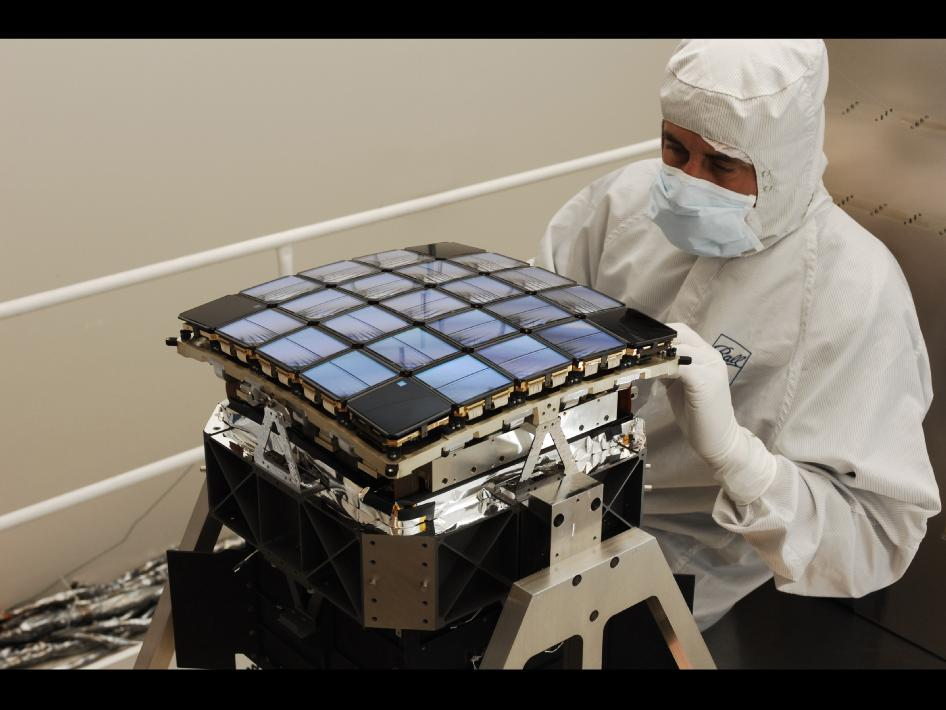
\includegraphics[width=0.45\linewidth]{Chapter1/Kepler_detector.jpg}
    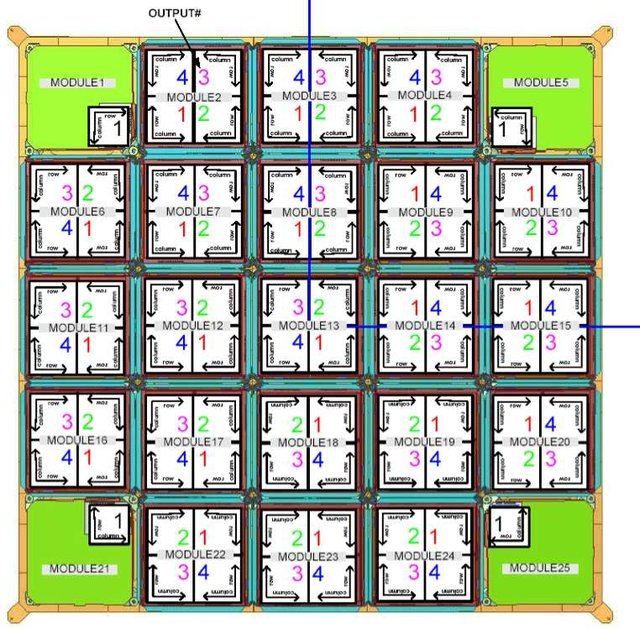
\includegraphics[width=0.45\linewidth]{Chapter1/kepCCD.jpg}
    \caption[Kepler CCD detector array prior to installation]{Left: The focal plane array assembly showing the 42 CCDs that comprised the detector at Bell Labs prior to launch. Right: A schematic of the detector module placements and identification of each module and output. Module positions 1, 5, 21, and 25 are occupied with fine guidance sensor chips. Credit: Kepler Instrument Handbook}
    \label{fig:Kep_detect}
\end{figure}

\subsection{Mission}
For the nominal mission, \Kepler~observed a 105 square degree field of view (FoV) centred between the constellations of Cygnus and Lyra, and located 13.5 degrees above the Galactic plane. Figure \ref{fig:kepFoV} shows the telescope's nominal FoV, with stellar magnitudes represented by the size of the filled circles. The four open clusters are marked by dashed circles. Note that the detector is positioned to ensure the brightest stars are focused between the modules to minimise blooming (overexposure and charge-bleeding along CCD rows). The telescope was intentionally defocused to diffuse the light of a stellar target to 10\," to ensure the best possible photometric stability \citep{gould_sensitivity_2003}.

\begin{figure}[htbp]
    \centering
    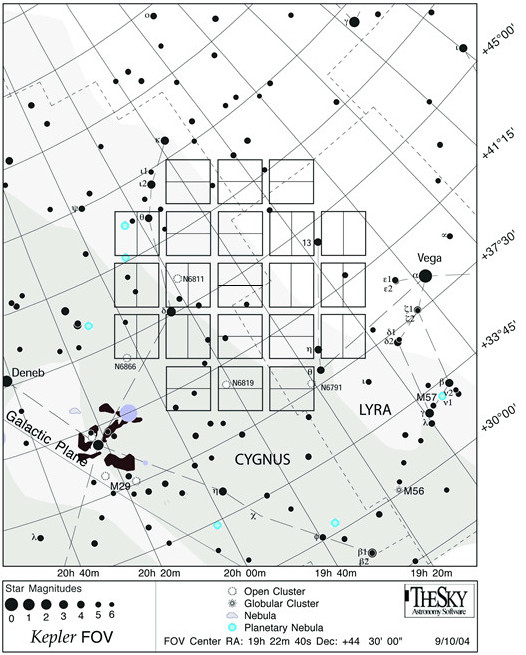
\includegraphics[height=0.32\paperheight]{Chapter1/kepFoV.jpg}
    \vspace{0.5em}
    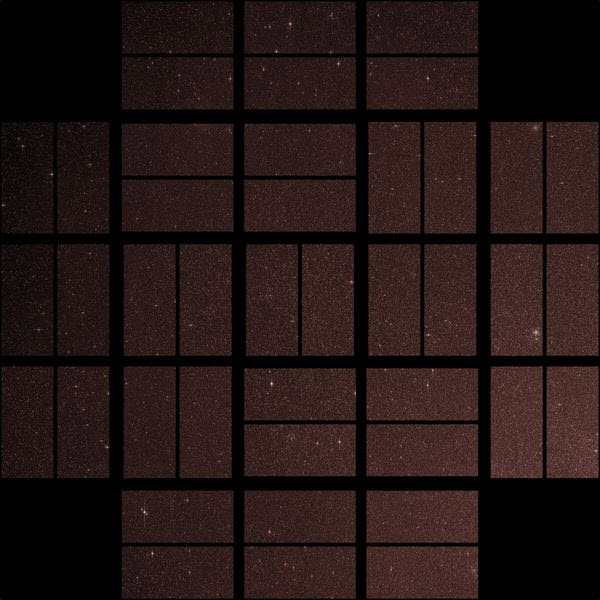
\includegraphics[width=0.45\linewidth]{Chapter1/kepFFI.jpg}
    \caption[\Kepler field of view; stylised, and full-frame image]{Left: Stylised representation of the \Kepler\, field of view between the constellations of Cygnus and Lyra. Larger filled circles represent stars of brighter magnitude. The four open clusters in the FoV are designated by dashed circles. Right: An example of the full-frame images (FFIs) of \Keplers~FoV.}
    \label{fig:kepFoV}
\end{figure}

\Kepler~occupied an Earth-trailing heliocentric orbit with the field of view selected to avoid Earth-shine, Moon-shine, and sunlight from entering the photometer. %One of the characteristics of an ETHO are lower torques acting on the spacecraft, enabling more efficient fine-pointing control. This control is achieved through the four reactor wheels that spin up to store the angular momentum from the acting torques before being dumped through thruster burns. 
The orbit also required the spacecraft to rotate every 90\,days to maintain sunlight on the solar array and prevent sunlight entering the telescope, placing stars on different CCDs. This rotation resulted in data being divided into "quarters" at each rotation. The initial 30\,d observing run (following the 10\,d engineering test but prior to the first rotation) is termed quarter 1 (Q1), with the nominal mission terminating after Q17 due to the failure of a second reaction wheel. These observations provide baseline photometry for most target stars of approximately 1\,460\,days.

\subsection{Data Products}
\label{chap:intro:data}

\Keplers on-board storage was limited, preventing the storage of full-frame images (FFIs) of the entire FoV between subsequent down links, at the cadence required for the mission's science goals \citep{bryson_Selecting_2010}. As a result, many small subsets of these images were selected for down-link, with only a single FFI (Figure \ref{fig:kepFoV}) downloaded every 30\,days \citep{thompson_kepler_2016}. All data products from the mission preserved pixel-level data, so subsets could be queried per pixel. Module 3 of the CCD detector failed in January 2010, so all stars that fell on this module, including NGC\,6819, have data gaps every four quarters that correspond to the spacecraft's rotation.

\subsubsection{Target Pixel Files}
The primary data products consisted of subsets or `postage stamps' of the CCD array output around target stars, called target pixel files (TPFs), and were produced for around 150\,000 targeted stars per quarter. \cite{batalha_selection_2010} selected stars so that Earth-sized planets ($\mathrm{R} \leq 2\mathrm{R_{\Earth}}$), if present, would be detectable in over 90\% of the targets. These included over 90\,000 G-type, main-sequence stars brighter than 16th magnitude, as well as $\sim 3000$ M-type main-sequence stars and $\sim 200$ O and B type stars. In addition, all known eclipsing binaries in the field of view, high proper motion stars, and some known cluster members were selected, with a limited number of slots reserved for guest observer proposed targets. There were two observational cadences for the TPFs: long cadence (LC) observations, with a total integration time of 29.43\,mins, and a smaller subset of approximately 500 short cadence (SC) observations, with an integration time of 58.86\,s. These were stored in on-board memory until down-link, every 30\,days. 

\subsubsection{Superstamp Images}
In addition to the primary data products, two large 200 $\times$ 200\,pixel `superstamps' centred on the open clusters NGC\,6791 and NGC\,6819 were downloaded at LC exposure intervals for quarters 1 to 17. These superstamps provide the opportunity to extract data for the non-targeted stars that comprise the majority of the crowded cluster centres, as well as allowing for the extraction of additional data for those stars that were either added to the guest observer list later in the \Kepler{} mission, or were removed to preference other stars. Figure \ref{fig:SS} shows a typical superstamp image for each cluster. NGC\,6819 fell on module 3 of the detector from Q2, so no superstamps are available for this cluster for Q6, Q10 or Q14.

\begin{figure}[htbp]
    \centering
    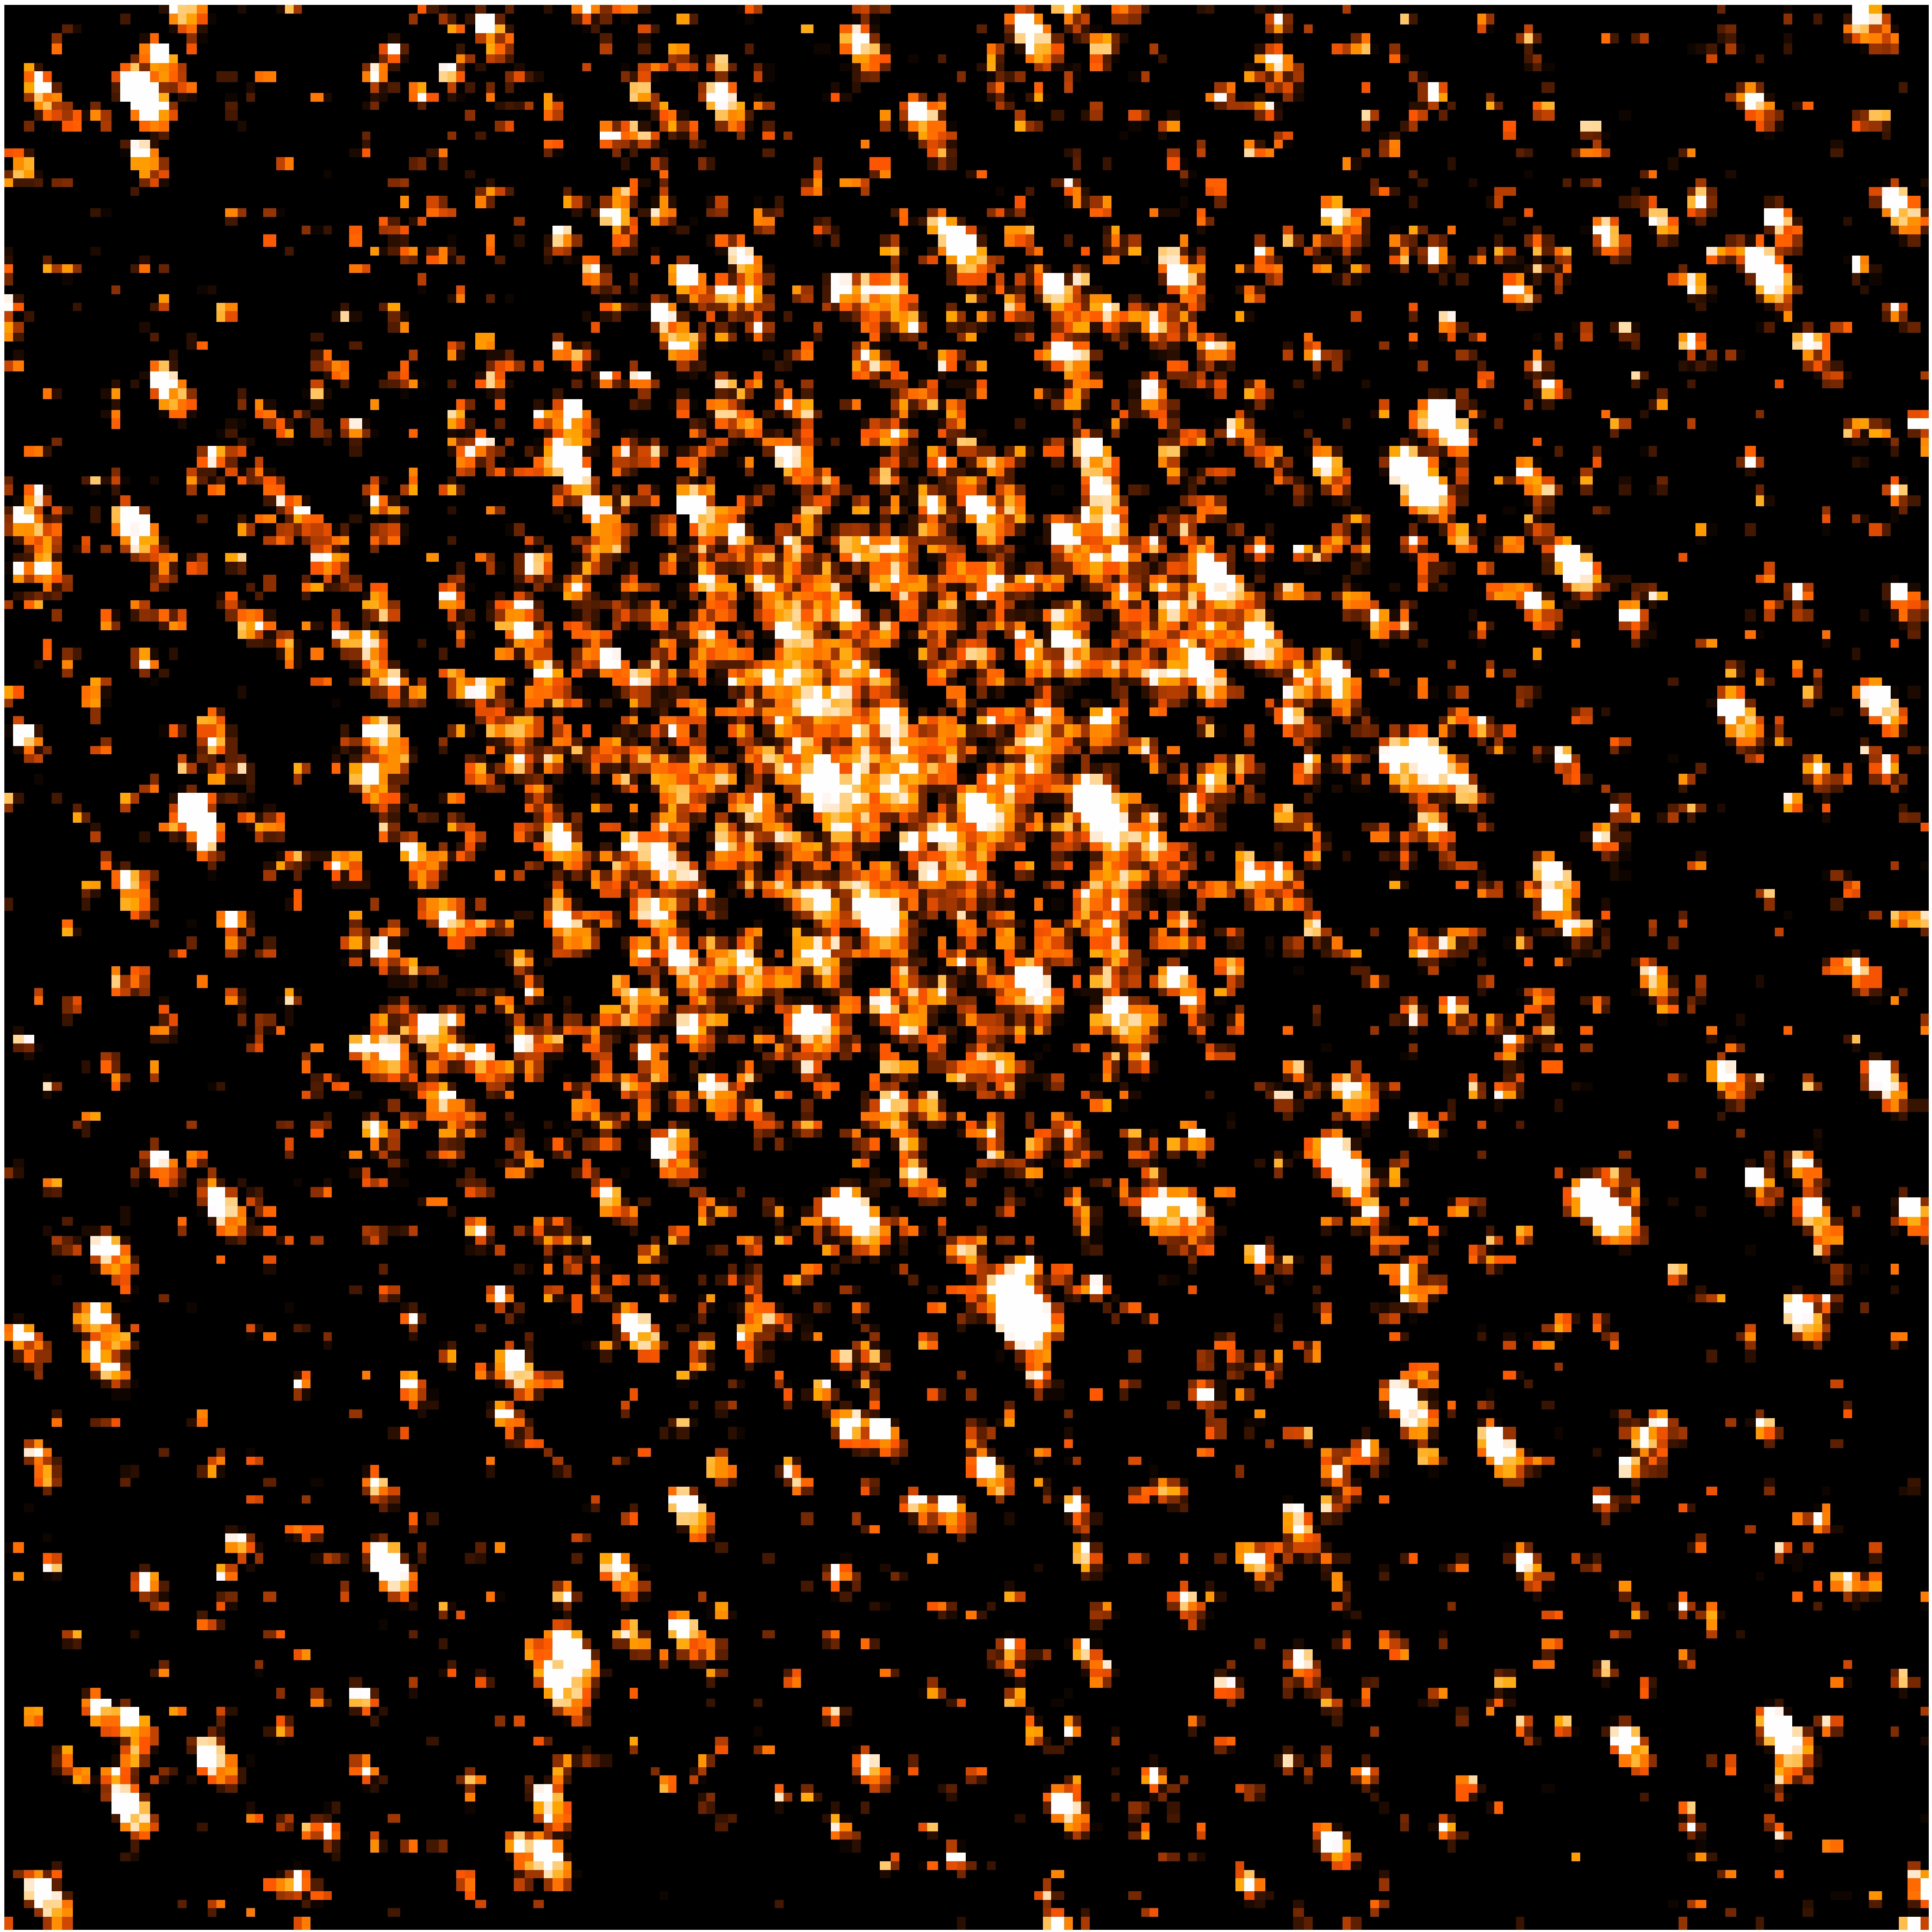
\includegraphics[width=0.45\linewidth]{Chapter1/ngc6791.jpg}
    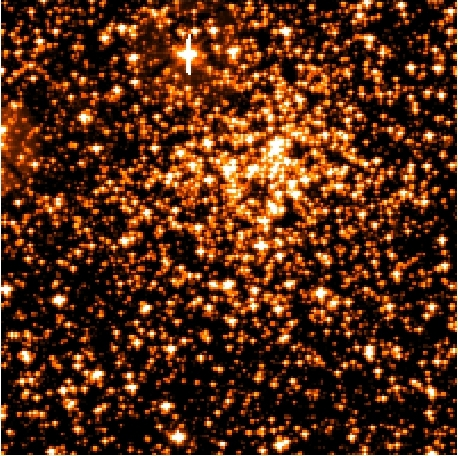
\includegraphics[width=0.45\linewidth]{Chapter1/ngc6819.jpeg}
    \caption[Superstamps of NGC\,6791 and NGC\,6819]{Typical superstamp images of the cores of the open clusters NGC\,6791 (left) and NGC\,6819 (right). The superstamps are 200 $\times$ 200\,pixels, corresponding to 13.27 $\times$ 13.27\,arcmins.}
    \label{fig:SS}
\end{figure}

% \newpage
% \section*{Outline of Thesis}

% Chapter 2 describes the stellar photometry we extracted from \Kepler~superstamp images of the open clusters of NGC\,6791 and NGC\,6819, as well as basic properties of these variable stars. In Chapter 3 we study one of these variables, KIC\,2569073, in greater depth, classifying its variability type and presenting its suitability for future investigations of Ap magnetic fields. Chapter 4 presents \Gaia~astrometric membership determinations for all stars within the fields of view of the nominal \Kepler~mission open clusters. In Chapter 5 we investigate the red giant solar-like oscillators as an ensemble, based on this membership. Finally, we summarise the key results of these investigations and provide avenues for future work in Chapter 6.

%From honours thesis:
%"long, well-sampled time series with high accuracy in the measurements, are also critical for asteroseismic studies."
 




% Murphy Thesis
% Asteroseismology is the most informative method with which we can observe the
% stellar interior. Other than solar neutrinos, it is the only method. Oscillation fre-
% quencies present in stars’ light curves are the fundamental data of asteroseismology,
% and permit us to fine-tune stellar models. Although ground-based support is still
% required, particularly in constraining stellar atmospheric parameters and for direct
% mode identification, the existence of nearly continuous, micromagnitude-precision,
% space-based photometry is revolutionising our capacity to study stars.


%----------------------------------------------------------------------------------------------------------------------------------------------------------------
%----------------------------------------------------------------------------------------------------------------------------------------------------------------